\section{Oratorio in rinnovo}

\begin{figure*}[!b]
  \begin{minipage}{0.1\textwidth}
    ~
  \end{minipage}
  \begin{minipage}{0.26\textwidth}
    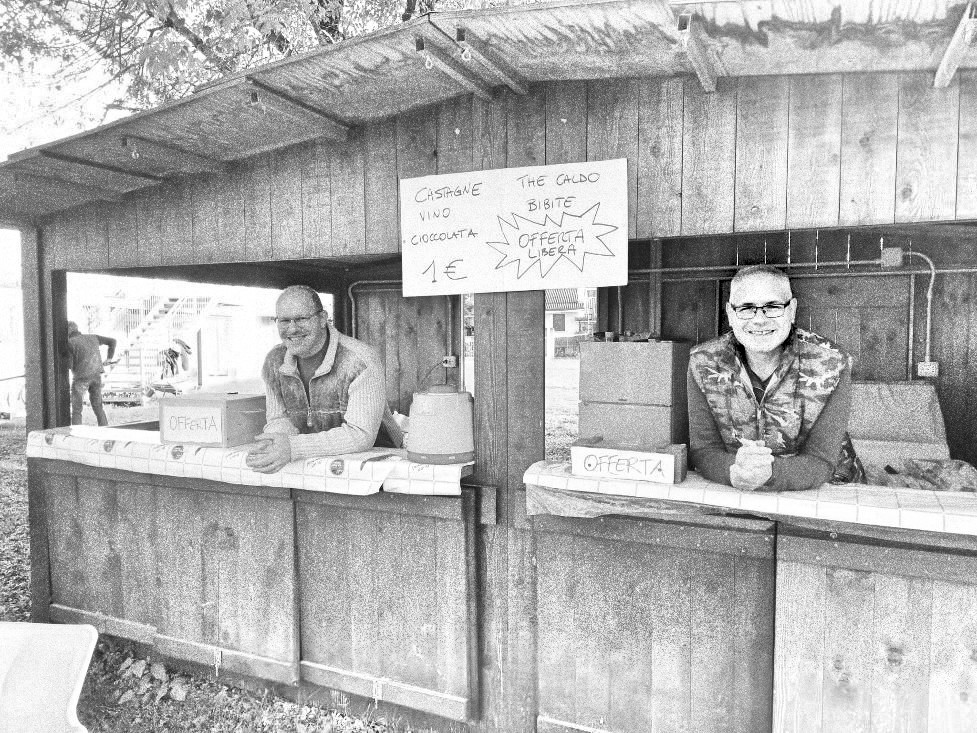
\includegraphics[width=\textwidth]{oratorio}
  \end{minipage}
  \hfill
  \begin{minipage}{0.44\textwidth}
    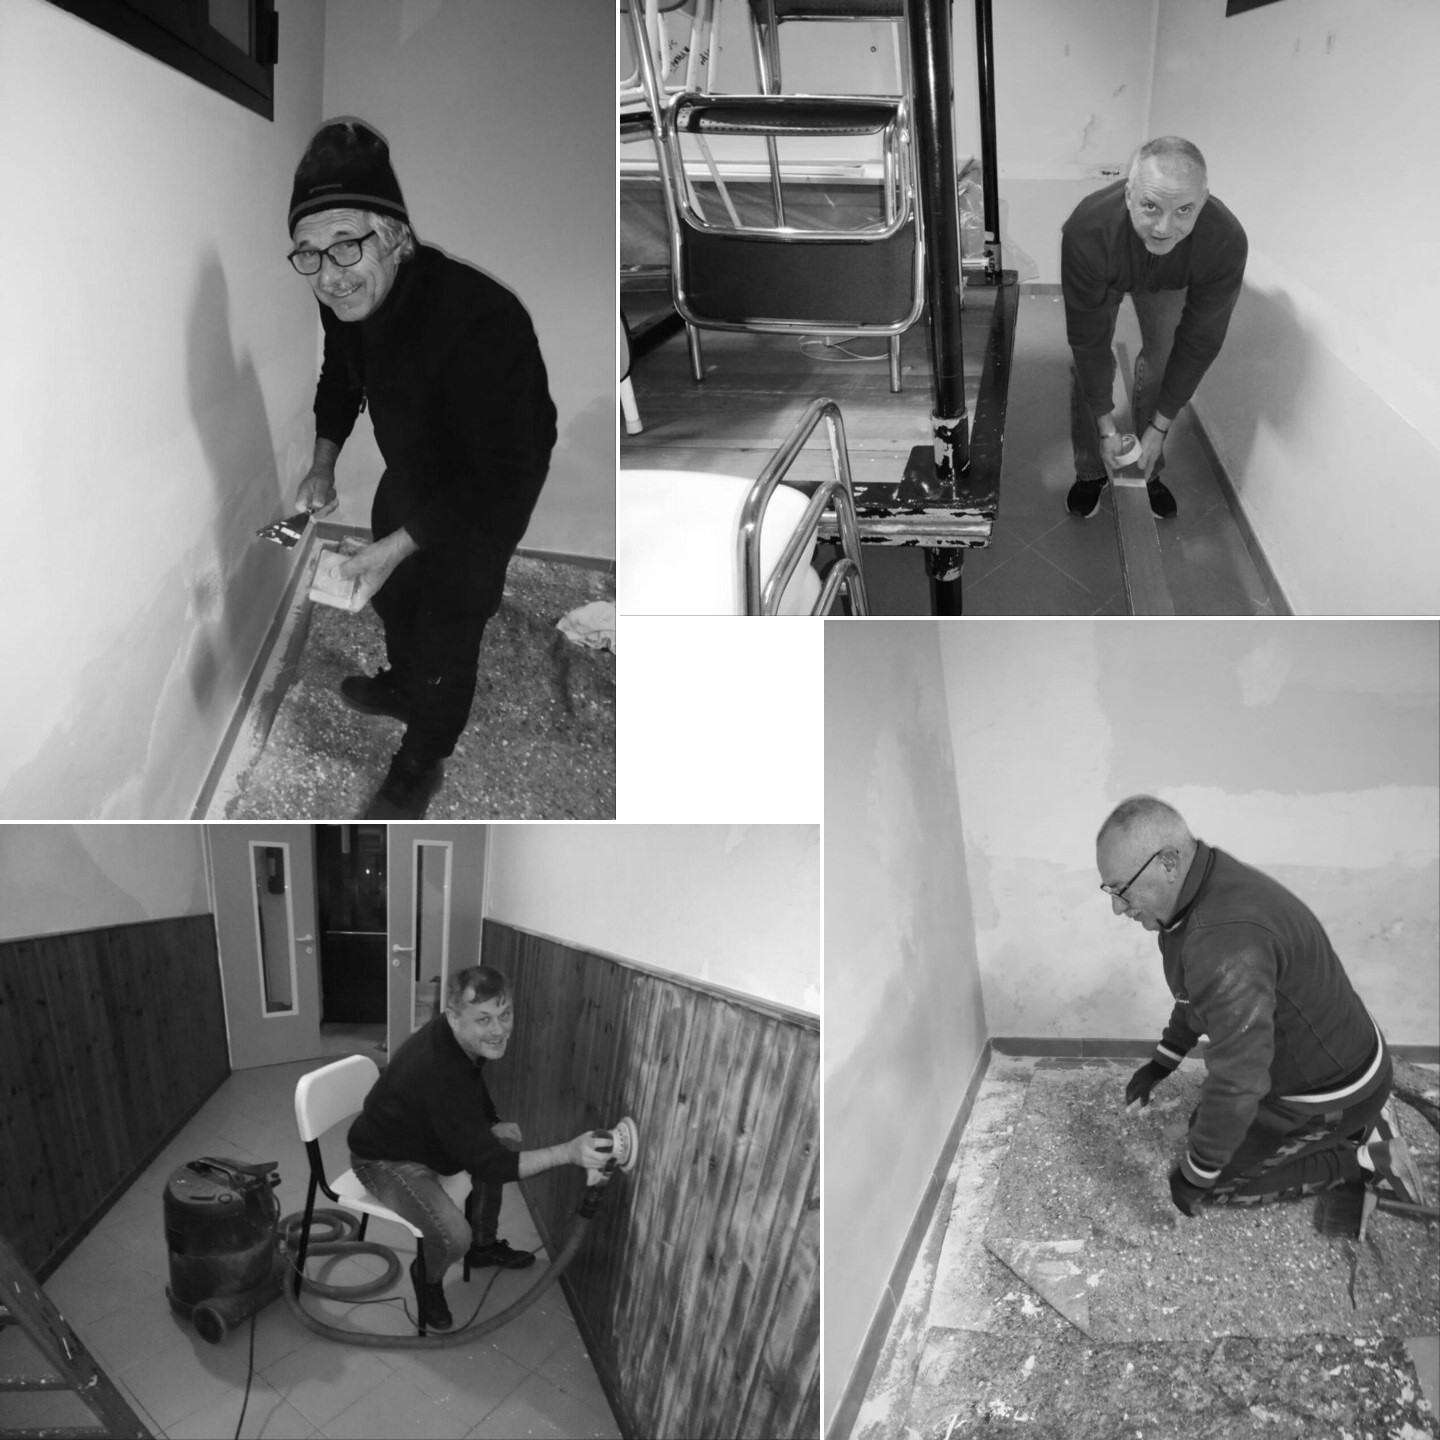
\includegraphics[width=\textwidth]{oratorio-all}
  \end{minipage}
  \begin{minipage}{0.1\textwidth}
    ~
  \end{minipage}
\end{figure*}

Sono cominciati oramai da mesi i lavori per il ripristino e rinnovo interno delle stanze del nostro oratorio San Giorgio. Dopo il rifacimento esterno continua il lavoro internamente da parte del Gruppo Oratorio Rinnovato formato da volontari, dal Gruppo Pesca, Gruppo Oratorio, Catechiste, Grest che con Don Mirco avevano convenuto l’esigenza di ristrutturare le stanze sottostanti, per il bene di tutti i bambini, ragazzi e gruppi che lo frequentano.

Così con l’aiuto di imbianchini professionisti e volontari è stato ultimato il corridoio rinfrescato da nuove tinte, con porte a norma di legge e controsoffittature per ogni stanza.

Il tutto ultimato in tempo perché il nostro caro Don Mirco potesse vederlo nel giorno del suo saluto alla Comunità e portasse con sé un bel ricordo del suo oratorio.

È prevista a breve la tinteggiatura di 5 stanze, dell’ingresso e il rinnovo dell’illuminazione con lampade più moderne ed efficienti, infine un probabile cambiamento della vecchia cucina. L’iniziativa è di questi gruppi parrocchiali composti da volontari che stanno dedicando forze ed energie, insieme al nostro nuovo parroco Don Federico che ha approvato i lavori, ma naturalmente per chiunque volesse unirsi alle squadre e regalare un po’ del suo tempo, è bene accetto. vi aspettiamo!

\firma{Buon Santo Natale dal Gruppo Oratorio Rinnovato \\ e da parte di tutti i gruppi e volontari}
